\section{单频波的程序}
我们将按他的启示行事。你的第一个问题与图\ref{fig:new/fig-2-3-1}所示之计算机程序有关。照实际情形来说,它将产生通过某一能量的波动传播的活动电影
(三维矩阵形式)。从编辑到计算直至最终看见循环影片的整个过程,约为一分钟(当你是计算机仅有的用户的时候)。
\subsection{循环影片程序之分析}
要使循环影片对观众有意义,电影的主题必须是周期性的,从而必须安排得使最后的
面很自然地与第一个画面衔接起来。在图\ref{fig:new/fig-2-3-1}所示程序形成的电影中,有一个参量
lambda,它控制着从顶部照亮屏幕之波动脉冲的基本重复率。当一个子波往下传播了四分
之一画面的路程时,另一个子波就应送进去。这种过程由下列一行程序来规定
\begin{equation*}
lambda=nz*dz/4=\frac{N_z\Delta_z}{4}
\end{equation*}
各脉冲均由频率为$n\omega$、即$\Delta \omega$、$2\Delta\omega\ldots\ldots$,$n\omega\Delta\omega$等之正弦波叠加而形成,最低频率$d\omega=\Delta\omega$
具有与lambda呈反比的波长。因此规定
\begin{equation*}
d\omega=v\times\pi^2/lambda=\frac{2\pi v}{\lambda}
\end{equation*}
最后,循环影片的延续时间必须等于最低频正弦波的周期
\begin{equation*}
N_t\Delta t=\frac{2\pi}{\Delta \omega}
\end{equation*}
最后这个方程定义了关于扫描线的时间间隔
\begin{equation*}
dt=\pi^2/(nt\times d\omega)
\end{equation*}
该程序所求解的偏微分方程为
\begin{equation}
\frac{\partial P}{\partial z}=\frac{i\omega}{v(x,z)}P+\frac{v}{-i\omega^2}\frac{\partial^2 P}{\partial x^2}
\label{eq:ex2.3.1}
\end{equation}
对于每个步长$\Delta z$,完成两步计算,第一步是解
\begin{equation}
\frac{\partial Q}{\partial z}=\frac{v}{-i\omega^2}\frac{\partial^2 Q}{\partial x^2}
\label{eq:ex2.3.2}
\end{equation}
利用Crank-Nicolson差分方法,此式变为
\begin{equation*}
\frac{q_{z+1}^x-q_z^x}{\Delta z}=-\frac{v}{i\omega^2}[\frac{q_z^{x+1}-2q_z^x+q_z^{x-1}}{2\Delta x^2}+
\frac{q_z^{x+1}-2q_{z+1}^x+q_{z+1}^{x-1}}{2\Delta x^2}]
\end{equation*}
将所有常数减缩成一个常数,并定义:
\begin{equation}
\alpha=\frac{v\Delta z}{-i\omega^4\Delta x^2}
\label{eq:ex2.3.3}
\end{equation}
得到
\begin{equation*}
q_{z+1}^x-q_z^x=\alpha[q_z^{x+1}-2q_z^x+q_z^{x-1}+q_z^{x+1}-2q_{z+1}^x+q_{z+1}^{x-1}]
\end{equation*}
将各未知数置于左端,则
\begin{equation}
-\alpha q_{z+1}^{x+1}+(1+2\alpha)q_{z+1}^x-\alpha q_{z+1}^{x-1}=\alpha q_z^{x+1}+(1-2\alpha)q_z^x+
\alpha q_z^{x-1}
\label{eq:ex2.3.4}
\end{equation}
\begin{figure}[H]
\centering
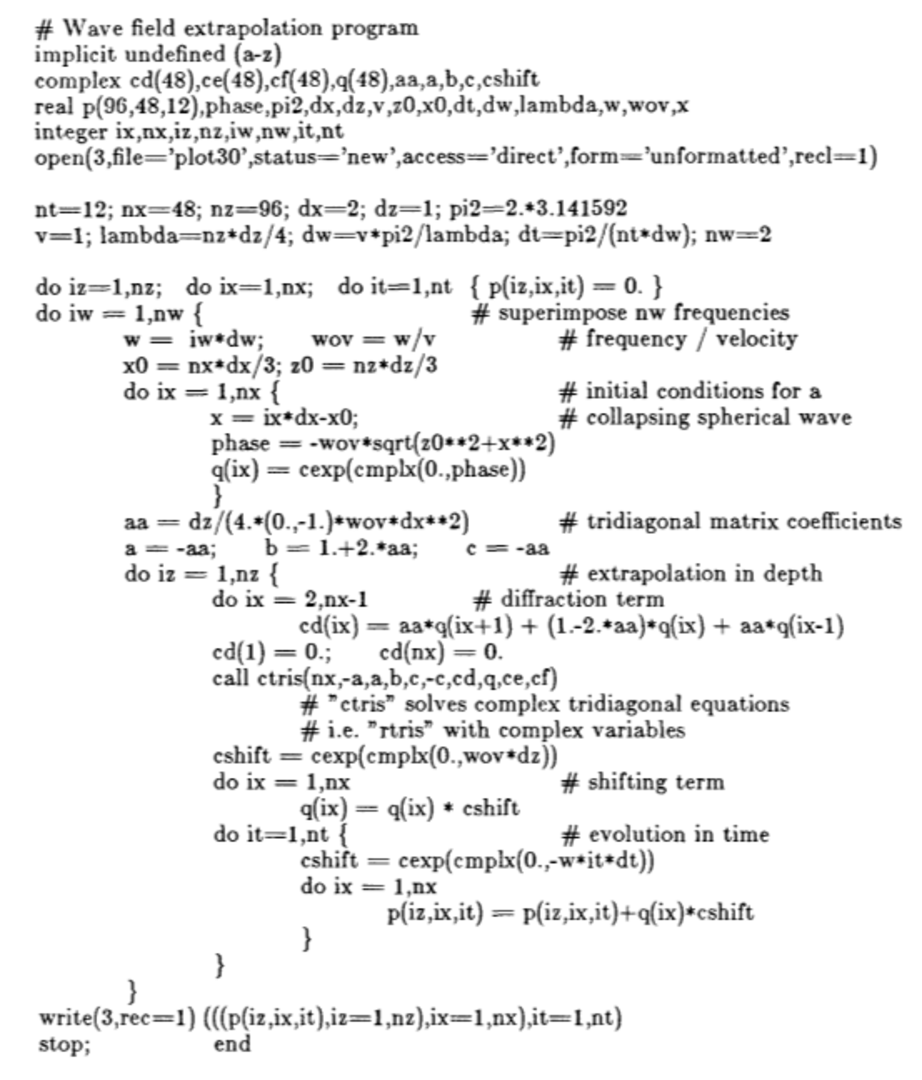
\includegraphics[width=0.85\textwidth]{new/fig-2-3-1}
\caption[code2-3-1]{产生单频波之和的电影的计算机程序}
\label{fig:new/fig-2-3-1}
\end{figure}
